\documentclass[11,a4paper,roman]{moderncv}
\moderncvstyle{banking}
\moderncvcolor{blue}
\usepackage[utf8]{inputenc}
\usepackage{polski}
\usepackage[polish]{babel}
\usepackage[scale=0.90]{geometry}
\usepackage{graphicx}
\makeatletter
\@ifpackageloaded{moderncvstylebanking}{%
\let\oldmakecvtitle\makecvtitle
\renewcommand*{\makecvtitle}{
  {\centering\framebox{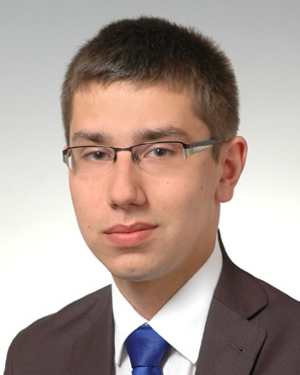
\includegraphics[width=75pt]{pic.jpg}}\par\vspace{5pt}}
  \oldmakecvtitle%
}%
}{%
}
\nopagenumbers
\makeatother

\def \polishskill {ojczysty} 
\def \englishskill {C2 / biegły} 
\def \germanskill {A2 / podstawowy} 
\def \frenchkill {A1 / podstawowy} 

\firstname{Kacper}
\familyname{Kasztelanic}
\title{Programista}
\email{k.kasztelanic@gmail.com}
\mobile{+48 793 954 321}
\social[github][github.com/kacperkasztelanic]{/ kacperkasztelanic}
\address{Wrocław}{}

\begin{document}
\makecvtitle
\vspace{-1,0cm}

\section{Wykształcenie}
\cventry{10/2015-teraz}{Studia inżynierskie na kierunku Informatyka}{Politechnika Wrocławska}{Wydział Informatyki i Zarządzania}{}{}
\cventry{02/2016-teraz}{Studia magisterskie na kierunku Budownictwo}{Politechnika Wrocławska}{Wydział Budownictwa Lądowego i Wodnego}{}{}
\cventry{10/2012-01/2016}{Studia inżynierskie na kierunku Budownictwo - stopień inżyniera}{Politechnika Wrocławska}{Wydział Budownictwa Lądowego i Wodnego}{}{}

\section{Narzędzia IT}
\cvitem{Java SE}{Java8, Collections, Multithreading, JDBC, Swing, Apache Libraries}
\cvitem{Java EE}{Servlets, JSP}
\cvitem{RDBS/SQL}{MySQL, SQLite}
\cvitem{Python}{OOP, numpy}
\cvitem{C++}{OOP, STL}
\cvitem{}{\textbf{Android}}

\section{Umiejętności techniczne}
\cvitem{Systemy operacyjne}{GNU/Linux, Windows}
\cvitem{System kontroli wersji}{GIT}
\cvitem{Techniki programowania}{Wzorce projektowe, SOLID}
\cvitem{Testy jednostkowe}{JUnit}
\cvitem{}{\textbf{Projektowanie relacyjnych baz danych}}

\section{Języki}
\cvlanguage{Polski}{\polishskill}{}
\cvlanguage{Angielski}{\englishskill}{}
\cvlanguage{Niemiecki}{\germanskill}{}
\cvlanguage{Francuski}{\frenchkill}{}

\section{Zainteresowania}
\cvitem{} {Optymalizacja oprogramoawania, sieci komputerowe, sprzęt komputerowy}
\cvitem{} {Lingwistyka, literatura angielska, muzyska, psychologia}
\vspace*{\fill}
\textit{\scriptsize Wyrażam zgodę na przetwarzanie moich danych osobowych dla potrzeb niezbędnych do realizacji procesu rekrutacji (zgodnie z Ustawą z dnia 29.08.1997 roku o Ochronie Danych Osobowych; tekst jednolity: Dz. U. 2016 r. poz. 922)..}
\end{document}
